% !TEX encoding = UTF-8 Unicode
\documentclass[a4paper]{article}

\usepackage{color}
\usepackage{url}
\usepackage[T2A]{fontenc} % enable Cyrillic fonts
\usepackage[utf8]{inputenc} % make weird characters work
\usepackage{graphicx}

\usepackage[english,serbian]{babel}
%\usepackage[english,serbianc]{babel} %ukljuciti babel sa ovim opcijama, umesto gornjim, ukoliko se koristi cirilica

\usepackage[unicode]{hyperref}
\hypersetup{colorlinks,citecolor=green,filecolor=green,linkcolor=blue,urlcolor=blue}

\usepackage{listings}
\usepackage{listings-golang}

%\newtheorem{primer}{Пример}[section] %ćirilični primer
\newtheorem{primer}{Primer}[section]

\definecolor{mygreen}{rgb}{0,0.6,0}
\definecolor{mygray}{rgb}{0.5,0.5,0.5}
\definecolor{mymauve}{rgb}{0.58,0,0.82}

\lstset{ 
  backgroundcolor=\color{white},   % choose the background color; you must add \usepackage{color} or \usepackage{xcolor}; should come as last argument
  basicstyle=\scriptsize\ttfamily,        % the size of the fonts that are used for the code
  breakatwhitespace=false,         % sets if automatic breaks should only happen at whitespace
  breaklines=true,                 % sets automatic line breaking
  captionpos=b,                    % sets the caption-position to bottom
  commentstyle=\color{mygreen},    % comment style
  deletekeywords={...},            % if you want to delete keywords from the given language
  escapeinside={\%*}{*)},          % if you want to add LaTeX within your code
  extendedchars=true,              % lets you use non-ASCII characters; for 8-bits encodings only, does not work with UTF-8
  firstnumber=1,                % start line enumeration with line 1000
  frame=single,	                   % adds a frame around the code
  keepspaces=true,                 % keeps spaces in text, useful for keeping indentation of code (possibly needs columns=flexible)
  keywordstyle=\color{blue},       % keyword style
  language=Golang,                 % the language of the code
  morekeywords={*,...},            % if you want to add more keywords to the set
  numbers=left,                    % where to put the line-numbers; possible values are (none, left, right)
  numbersep=5pt,                   % how far the line-numbers are from the code
  numberstyle=\tiny\color{mygray}, % the style that is used for the line-numbers
  rulecolor=\color{black},         % if not set, the frame-color may be changed on line-breaks within not-black text (e.g. comments (green here))
  showspaces=false,                % show spaces everywhere adding particular underscores; it overrides 'showstringspaces'
  showstringspaces=false,          % underline spaces within strings only
  showtabs=false,                  % show tabs within strings adding particular underscores
  stepnumber=1,                    % the step between two line-numbers. If it's 1, each line will be numbered
  stringstyle=\color{mymauve},     % string literal style
  tabsize=2,	                   % sets default tabsize to 2 spaces
  title=\lstname                   % show the filename of files included with \lstinputlisting; also try caption instead of title
}



\begin{document}

\title{Uvod u programski jezik Go\\ \small{Seminarski rad u okviru kursa\\Metodologija stručnog i naučnog rada\\ Matematički fakultet}}

\author{Luka Marković, Tamara Radovanović, Rade Aleksić, Milan Pužić\\ luka.markovic.d@gmail.com, radovanovic.tamara.t@gmail.com,\\ aleksic0rade@gmail.com, milanpuzic@gmail.com
}

\date{5.~april 2019.}

\maketitle


\abstract{
Ovaj rad je posvećen programskom jeziku Go. On spada u mlade jezike sa jednostavnim i čitljivim kodom. U ovom radu biće prikazane osnove jezika Go, njegova sintaksa i neki primeri koda. U prvom delu ćemo se osvrnuti na razvoj jezika i  radno okruženje. Nakon toga biće reči o osnovnim delovima programa pisanih u Go jeziku. Za sam kraj biće predstavljeno na koji način Go ostvaruje konkurentno programiranje.
}

\tableofcontents

\newpage

\section{Uvod}
\label{sec:uvod}

Go je programski jezik opšte namene, razvijen u kompaniji Google. Ideja je bila osmišljavanje novog, jednostavnog i moćnog jezika. Go je imperativni, statički tipizirani, kompajlirani jezik. Zbog svojih karakteristika za njega se kaže da je C 21 veka \cite{TheWaytoGo}. On nije objektno orijentisan, ali preuzima neke od koncepata iz objektno orijentisanih jezika kao što su metodi koji se dodeljuju korisnički definisanim tipovima i interfejsi. Go je dobar za izradu serverskih apikacija, zbog svoje konurentosti. Zbog svih ovih karakteristika postao je popularan u kratkom vremenskom periodu. 

\section{Nastanak i razvoj}
\label{sec:nastanak_i_razvoj}

U ovoj glavi će biti opisani razlozi za nastanak jezika Go, koji su jezici uticali na njegov razvoj, kao i neke osnovne karakteristike i namene.

\subsection{Istorija}
\label{subsec:istorija}

Programski jezik Go je nastao 2007. godine i kao takav spada u mlade programske jezike. Javno je predstavljen 2009. godine kao projekat otvorenog koda nastao unutar kompanije Google. Jezik su osmislili Robert Griesemer, Rob Pike i Ken Thompson, a njihov osnovni cilj bio je da naprave novi jezik opšte namene. Go je nastao kao pokušaj da se ukombinuju lak način pisanja i čitanja interpretiranih jezika i efikasnost i sigurnost jezika koji se kompajliraju.

Go je nastao pod uticajem raznih jezika, preuzimajući njihove ideje i izbegavajući karakteristike koje dovode do komplikovanog koda. Može se reći da pripada familiji programskog jezika C, iako je koncept konkurentnosti preuzeo iz Limbo i Newsqueak jezika. Mesto Go jezika u razvojnom stablu se može videti na slici \ref{fig:razvojno_stablo}. Slična sintaksa, ali znatno pojednostavljena i čistija u odnosu na jezik C, omogućila je velikom broju programera da se lako upoznaju sa ovim jezikom. \cite{TheGoProgramingLanguage}

\begin{figure}[htbp]
\begin{center}
    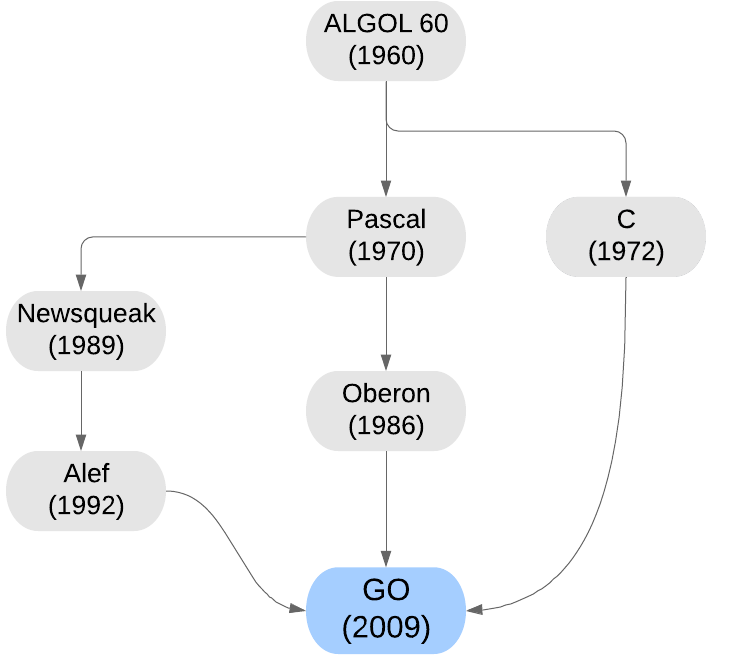
\includegraphics[scale=0.4]{razvojno_drvo.png}
    \caption{Razvojno stablo}
    \label{fig:razvojno_stablo}
\end{center}
\end{figure}

\subsection{Karakteristike}
\label{subsec:karakteristike}

Programeri koji su dizajnirali Go su želeli jednostavan jezik. Iz tog razloga, napravljen je jezik koji nije objektno orjentisan. U Go-u ne postoje klase, koncept nasleđivanja kao ni konstruktori, izuzeci ili anotacije. To Go čini drugačijim od drugih jezika. 

Kako bi olakšali programiranje, Go ima automatsko upravljanje memorijom, odnosno sakupljnje otpada. Iako statički tipiziran, preuzeo je i karakteristike dinamički tipiziranih jezika kao što su Python i Ruby.  Kako je nastao u eri multiprogramiranja, Go omogućava efikasnu konkurentnost koja je ugrađena u sam jezik. Go podržava gorutine umesto niti. One zazuimaju oko 2KB memorije, što je mnogo manje nego 1MB koliko zauzima svaka nit u Javi. Sve ovo čini Go brzim i moćnim jezikom \cite{article}.



\subsection{Instalacija i korisničko okruženje}
\label{subsec:karakteristike1}

Kako bismo programirali koristeći programski jezik Go, sve što nam je potrebno su tekst editor i kompajler za Go.

Može se koristiti bilo koji tekst editor, s tim što bi bilo poželjno da podržava sintaksu programskog jezika Go. Za većinu text editora moguće je instalirati paket koji omogućava lakše pisanje koda.

Bilo da koristite Windows, Linux ili macOS, poslednju verziju kompajlera za Go kao i uputstvo za instalaciju možete naći na zvaničnoj strani Go jezika \cite{golang}.

Ekstenzija izvornog koda programa napisanog u Go jeziku je .go, a nakon njegove kompilacije dobija se izvršni kod sa ekstenzijom .out na Unix i .exe na Windows operativnim sistemima. 

Programi pisani u jeziku Go se takođe mogu pisati u razvojnom okruženju. Postoji više razvojnih okruženja među kojima je najpoznatije GoLand \cite{GoLend}.



\section{Osnovna sintaksa}
\label{osnovna_sintaksa}

Pre nego što krenemo dalje da razmatramo osnovne elemente programskog jezika Go, pogledajmo prvo minimalnu strukturu za svaki program pisan u njemu.

Program pisan u Go-u u osnovi sadrži sledeće delove:
\begin{itemize}
\item Deklaraciju paketa
\item Uključivanje drugih paketa u naš program
\item Funkcije
\item Promenljive
\item Naredbe za kontrolu toka i naredbe grananja
\item Komentare
\end{itemize}

\begin{primer}
Pogledajmo jednostavan primer \ref{zdravo} koji na standardnom izlazu ispisuje poruku “Zdravo svete!”

\end{primer}
\begin{lstlisting}[caption={Zdravo svete},frame=single, label=zdravo]
package main
import "fmt"
func main() {
   fmt.Println("Zdravo svete!")
}
\end{lstlisting}

Prva linija programa definiše ime paketa u kome se program nalazi. Paket \texttt{main} je početna tačka za izvršavanje programa. Svaki paket ima pridruženu putanju i ime.
Sledeća linija je pretprocesorska komanda koja govori Go kompajleru da uveze fajlove koji se nalaze u paketu \texttt{fmt}.
Funkcija \texttt{main()} je funkcija od koje počinje izvršavanje programa. Kada operativni sistem pokrene program, on prvo poziva ovu funkciju.
Tekst ograničen karakterima \texttt{/*…*/} označava komentare u programskom jeziku Go. 
Komanda \texttt{Fmt.Println(\char`\"Zdravo, svete")} poziva funkciju \texttt{Println} iz paketa \texttt{fmt} koja ispisuje na standardni izlaz poruku “Zdravo svete”.

Naredbe u programskom jeziku Go se razdvajaju novim redom. Nije obavezno navoditi karakter \texttt{;} kao na primer u programskim jezicima C i Java. Moguće je napisati više naredbi u istom redu, ali se tada one moraju razdvajati karakterom \texttt{;}.

\subsection{Komentari i identifikatori}
\label{subsec:komentari_i_identifikatori}

Komentari u Go-u  mogu biti jednolijski ili višelinijski. Višelinijski komentari su ograničeni između sekvenci karaktera \texttt{/*} i \texttt{*/}. Jednolinijski komentari počinju sekvencom karaktera \texttt{//}.

\begin{lstlisting}[caption={Komentari},frame=single, label=komentari]
/* Ovo je komentar
koji se prostire
na vise linija */

// Ovo je jednolinijski komentar
\end{lstlisting}

Identifikatori su imena koja jednoznačno određuju promenljive, funkcije i sve ono što korisnik definiše. Imena identifikatora počinju velikim ili malim slovom ili karakterom \texttt{\_}, a zatim su opciono praćeni kombinacijom slova, brojeva i karaktera \texttt{\_}. Izvorne datoteke sa kodom su uvek kodirane sa UTF-8.

Validna imena identifikatora u Go programskom jeziku: 

\begin{lstlisting}[caption={Imenovanje identifikatora},frame=single, label=identifikatori]
imePromenljive     DrugoIme_promenljive     %*ћирилица*)30
\end{lstlisting}

Programski jezik Go razlikuje velika i mala slova (eng.  case-sensitive), što znači da su identifikator \texttt{foobar} i identifikator \texttt{FooBar} dva različita identifikatora.

Sledeća tabela \ref{tab:tabela1} prikazuje ključne reči u programskom jeziku Go. To su reči koje su rezervisane i ne mogu se upotrebljavati ni za imena promenljivih i konstanti, niti za bilo koji drugi identifikator.

\begin{table}[h!]
\begin{center}
\caption{Rezervisane reči u jeziku Go}
\begin{tabular}{|l|l|l|l|l|}
\hline
break    & default     & func   & interface & select \\ \hline
case     & defer       & Go     & map       & Struct \\ \hline
char     & else        & GoTo   & package   & Switch \\ \hline
const    & fallthrough & if     & range     & Type   \\ \hline
continue & for         & import & return    & Var   \\ \hline
\end{tabular}
\label{tab:tabela1}

\end{center}
\end{table}

\subsection{Promenljive i konstante - deklaracija i inicijalizacija}
\label{subsec:prom_i_konst}

Pomoću ključne reči \texttt{var} kreiramo promenljivu određenog tipa, dodeljujemo joj neko ime i inicijalizujemo vrednost. Svaka deklaracija promenljive ima sledeću formu: \lstinline{var ime tip = izraz}

Jedna od vrednosti \texttt{tip} ili \texttt{izraz} može biti izostavljena, ali nikako obe. Ako se izostavi \texttt{tip}, tip se dodeljuje na osnovu vrednosti izraza. Ako se izostavi \texttt{izraz}, onda se vrednost promenljive inicijalizuje na “nula” za određen tip. Za numeričke vrednosti to je \texttt{0}, za bulovske vrednosti to je \texttt{false}, za string \texttt{\char`\"\char`\"}, za referencne vrednosti to je \texttt{nil}.

“Nula vrednost” mehanizam obezbeđuje da svaka promenljiva u svakom trenutku ima validnu vrednost određenog tipa. Dakle, u programskom jeziku Go ne postoje neinicijalizovane promenljive.

Moguće je deklarisati i inicijalizovati više promenljivih u jednoj liniji. 
\begin{lstlisting}[caption={Inicijalizacija i deklaracija više promenljivih},frame=single, label=Inicijalizacija_i_deklaracija_vise_promenljivih]
var x, y, z Int // sve promenljive su tipa int i imaju vrednost 0
var x, y, z = 2, true, 0 // promenljive x i z su tipa int i imaju vrednost 2 i 0, a y je tipa bool i ima vrednost true
\end{lstlisting}


Unutar funkcija je moguće koristiti takozvanu kratku deklaraciju promenljivih koja ima oblik:
\lstinline{Ime := izraz}

Deklaracija je moguća i pomoću ključne reči \texttt{const}. U ovom slučaju sintaksa je slična onoj kod koje se koristi ključna reč \texttt{var}, ali definiše imenovanu vrednost čija vrednost mora da bude konstanta. Vrednost mora biti poznata u toku kompajliranja programa. Tip konstantne promenljive mora biti osnovni tip, odnosno numerička vrednost, bulovska vrednost ili string.

\lstinline{const pi = 3.14}

\section{Tipovi i strukture podataka}	
\label{sec:tipovi_i_strukture}

Go je statički tipiziran jezik što znači da se promenljivoj dodeljuje tip prilikom njene deklaracije i on se ne može menjati tokom izvršavanja programa. Tip promenljive se ne mora eksplicitno navesti, već se može zaključiti na osnovu dodele operatorom \texttt{:=} kada se promenljiva uvodi.

Tipovi podataka koji su definisani u programskom jeziku Go mogu se klasifikovati u četiri kategorije \cite{TheGoProgramingLanguage}:

\begin{enumerate}
\item Osnovni tipovi 
\item Složeni tipovi
\item Referentni tipovi 
\item Interfejsni tipovi 
\end{enumerate}




\subsection{Osnovni tipovi}
\label{subsec:osnovni_tipovi}

U osnovne tipove u programskom jeziku Go spadaju numerički, stringovski, i bulovski tipovi. Numerički tipovi uključuju nekoliko tipova celih brojava (eng. integer), brojeva sa pokretnim zarezom (eng. floating point) i kompleksnih brojeva.

Celi brojevi mogu da budu označeni i neoznačeni. Postoje 4 vrste celih  brojeva u programskom jeziku Go i oni su klasifikovani po veličini, preciznije memoriji koja je potrebna za njihovo čuvanje. To su reprezentacije celih brojeva od 8, 16, 32 i 64 bita i u Go-u se označavaju respektivno sa: \texttt{int8}, \texttt{int16} i \texttt{int32}, \texttt{int64} za označene brojeve i sa \texttt{uint8}, \texttt{uint16}, \texttt{uint32} i \texttt{uint64}  za neoznačene brojeve. 

Cele broje označavamo i sa samo \texttt{int} ili \texttt{uint} i ovi tipovi su predstavljeni u memoriji sa 32 ili 64 bita zavisno od hardvera. Operacije koje se mogu izvesti nad celim brojevima su prikazane u tabeli \ref{tab:tabela2}.


\begin{table}[h!]
\begin{center}
\caption{Aritmetičke i logičke operacije nad celim brojevima}
\begin{tabular}{|l|l|l|l|}
\hline
+    & Sabiranje  & *                                                       & Množenje \\ \hline
-    & Oduzimanje           & /                                                       & Deljenje           \\ \hline
\%   & Ostatak pri deljenju & ++                                                      & Inkrementacija      \\ \hline
--   & Dekrementacija       & ==                                                      & Ispitivanje jednakosti \\ \hline
!=   & Nejednakost          & \textgreater{},\textgreater{}=,\textless{},\textless{}= & Relacije veće, manje…       \\ \hline
\&\& & Logičko I            & ||                                                      & Logičko ili        \\ \hline
!    & Logička negacija     & =                                                       & Operator dodele    \\ \hline
\end{tabular}
\label{tab:tabela2}

\end{center}
\end{table}

U programskom jeziku Go postoje dva tipa brojeva sa pokretnim zarezom i označavamo ih sa \texttt{float32} i \texttt{float64}. Njihova fizička reprezentacija kao i aritmetičke operacije određene su IEEE 754 standardom čiju implementaciju podržava većina modernih procesora.
Postoje dve bulovske vrednosti u programskom jeziku Go, a to su \texttt{true} i \texttt{false}. Promenljive ili konstante koje čuvaju bulovsku vrednost su tipa \texttt{bool}.

Stringovi su nepromenljiva sekvenca bajtova. Stringovi mogu da čuvaju proizvoljne podatke, ali najčešće je to tekst razumljiv čoveku. Tekst stringova je predstavljen kao UTF-8 enkodirana sekvenca.
Stringovi su nepromenljivi (eng. immutable), što znači da sekvenca bitova nikada ne može biti promenjena. Na primer, ako imamo string \texttt{s} deklarisan sa \lstinline{s := "String"} i pokušamo da promenimo prvo slovo \lstinline{s[0] = 'R'}, dobili bismo grešku od strane kompajlera. Ako bismo uradili konkatenaciju dva stringa operatorom \texttt{+} i uradili sledeće \lstinline{s = s + "mutirani"}, ne bismo promenili prvobitni string \texttt{s}, već bi se napravio novi string \texttt{\char`\"String mutirani"} i dodelio promenljivoj \texttt{s}. \cite{IntroductionToProgrammingInGo}

\subsection{Složeni tipovi podataka}
\label{subsec:slozeni_tipovi}
U složene tipove podataka u programskom jeziku Go spadaju nizovi i strukture.

Niz je sekvenca, fiksne dužine, od 0 ili više elemenata istog tipa. Pojedinačnom elementu niza može se pristupiti preko njegovog indeksa. Indeksiranje u Go-u počinje od 0, što znači da prvi element u nizu ima indeks 0, drugi 1... 


\begin{lstlisting}[caption={Deklaracija nizova},frame=single, label=Deklaracija_nizova]
var a [3]int // deklaracija niza od tri cela broja
fmt.Println(a[0]) // Ispisuje prvi element na standardni izlaz
\end{lstlisting}


Podrazumevano, elementi niza su incijalno postavljeni na 0 ako se drugačije ne naglasi. 
Niz je moguće inicijalizovati prilikom deklaracije. 

\begin{lstlisting}[caption={Inicijalizacija niza prilikom deklaracije},frame=single, label=Inicijalizacija_niza_prilikom_deklaracije]
var niz [3]int = [3]int{1, 12, 3} // prvi element je 1, drugi 12, treci 3
\end{lstlisting}


Veličina niza je deo njegovog tipa, dakle niz \texttt{[3]Int} i niz \texttt{[4]Int} su različiti tipovi. Veličina mora biti konstantan izraz, čija vrednost može da se izračuna kada se program kompajlira. Sledeći izrazi daju grešku prilikom kompajliranja:

\begin{lstlisting}[caption={Primer greške sa nizovima},frame=single, label=Primer_greske_sa_nizovima]
q := [3]int{1, 2, 3}
q = [4]int{1, 2, 3, 4} // compile error: cannot assign [4]int to [3]int
\end{lstlisting}

Go dozvoljava poređenje nizova iste dužine definisanih nad istim tipom podataka, relacionim operatorima \texttt{==} i \texttt{!=}. Dva niza su jednaka ako imaju jednake vrednosti na istim pozicijama.


Struktura je tip podatka u programskom jeziku Go koja grupiše zajedno nula ili više različitih podataka. Svaki podatak ima svoje ime i svoju vrednost. Definisanjem strukture definiše se novi tip pomoću ključne reči \texttt{type}, zatim ide ime novog tipa, pa ključna reč \texttt{struct} i onda definicija strukture unutar zagrada \texttt{\{\}}. Pogledajmo primer:

\begin{lstlisting}[caption={Definicija strukture},frame=single, label=Definicija_strukture]
type Automobil struct {
	proizvodjac String,
	marka String,
	snaga Int	
}

var golf Automobil;
\end{lstlisting}

Pojedinačnim poljima se pristupa pomoću tačka notacije. U primeru iznad, kada bismo želeli da saznamo snagu automobila \texttt{golf}, uradili bismo sledeće: \texttt{golf.snaga}.
Ako je moguće uporediti polja strukture određenog tipa, onda je moguće uporediti i same strukture tog tipa operatorima \texttt{==} i \texttt{!=}.


\subsection{Referentni tipovi podataka}
\label{subsec:referentni_tipovi}


U referentne tipove podataka spadaju pokazivači, isečci, kanali, mape i  funkcije.

Pokazivači su vrsta podataka koji čuvaju memorijsku adresu neke promenljive. Dakle, pokazivač čuva lokaciju u memoriji na kojoj je sačuvan neki podatak imenovane promenljive. Pomoću pokazivača možemo da pristupamo i menjamo  vrednost promenljive bez znanja imena same promenljive. Ako je promenljiva deklarisana sa \texttt{var x int} onda operatorom \texttt{\&} možemo dobiti adresu promenljive \texttt{x}.

\begin{lstlisting}[caption={Primer pokazivača},frame=single, label=Primer_pokazivaca]
x := 1
p := &x // pokazivac na promenljivu x
\end{lstlisting}

Vrednost na koju pokazuje neki pokazivač možemo dobiti operatorom \texttt{*}. U primeru iznad, vrednost na koju pokazuje \texttt{p} dobijamo sa \texttt{*p}. Takvu vrednost možemo i da izmenimo naredbom \texttt{*p = 2}.
“Nula” vrednost za pokazivač na bilo koji tip je \texttt{nil}. Pokazivači su uporedivi, dva pokazivača su jednaka ako pokazuju na istu memorisku adresu ili ako su oba \texttt{nil}.
Pokazivače možemo da kreiramo i bez promenljive, izraz \texttt{new(E)} kreira neimenovanu promenljivu tipa \texttt{E}, inicijalizuje je na “nula” vrednost tipa \texttt{E} i vraća adresu te promenljive.

\begin{lstlisting}[caption={Primer kreiranja pokazivača},frame=single, label=Primer_kreiranje_pokazivaca]
p := new(int)  // p je tip *int , pokazuje na neku neimenovanu promenljivu
\end{lstlisting}


Isečak (eng. slice) čini sekvencu elemenata promenljive dužine, čiji elementi imaju isti tip. Isečak se označava sa \texttt{[]T}, gde elementi imaju tip \texttt{T}. Podseća na niz, samo bez unapred određene dužine. Isečak ima tri komponente: pokazivač, dužinu i kapacitet. Pokazivač pokazuje na prvi element u isečku. Dužina je broj elemenata u isečku i ona ne može da bude veća od kapaciteta. Dok je kapacitet alociran broj elemenata za isečak, odnosno broj elemenata za koji je rezervisan prostor u memoriji.

Kanali (engl. chan) omogućavaju dvosmernu komunikaciju između dve gorutine. Oni će biti detaljnije opisani u poglavlju \ref{sec:Konkurentno programiranje}.

U programskom jeziku Go, mapa je referentni tip podataka koja referiše na heš tabelu. Heš tabela je neuređena kolekcija sačinjena od parova ključ-vrednost. Mapa se označava sa \texttt{map[K]V}. \texttt{K} je tip ključa i on mora biti uporediv operatorom \texttt{==}, a \texttt{V} je tip vrednosti. Ključ mora da bude jedinstven za svaku vrednost u tabeli.
Pomoću funkcije \texttt{make} možemo da kreiramo jednu mapu.

\begin{lstlisting}[caption={Kreiranje mape},frame=single, label=Kreiranje_mape]
mapa = make(map[string]int) //Kljuc tipa string, a vrednost int
mapa["godine"] = 34
\end{lstlisting}

Mapa se može kreirati i na drugi način, gde joj se prilikom kreiranja inicijalizuje vrednost:

\begin{lstlisting}[caption={Inicijalizacija mape prilikom deklaracije},frame=single, label=Inicijalizacija_mape_prilikom_deklaracije]
godine := map[string]int{
"tamara": 24,
"milan": 23,
}
// kod iznad je ekvivalentan sa:
godine := make(map[string]int)
godine["tamara"] = 24
godine["milan"] = 23
\end{lstlisting}

Funkcije ćemo detaljnije predstaviti u poglavlju \ref{subsec:funkcije}.

\subsection{Interfejsni tipovi podataka}
\label{subsec:Inter_tipovi}

Interfejsi izražavaju apstrakciju ili generalizaciju ponašanja nekog drugog tipa. Pomoću generalizacije, intefejsi nam dozvoljavaju  da pišemo funkcije koje su fleksibilnije i adaptiranije zato što ne ulaze u detalje određene implementacije. O interfejsnim tipovima ćemo pisati u poglavlju \ref{subsec:interfejsi}.
\section{Kontrola toka}	
\label{sec:kontrola_toka}

\subsection{Naredbe grananja}
\label{subsec:naredbe_grananja}

U programskom jeziku Go razlikujemo dve naredbe grananja \texttt{if} odnosno \texttt{if else} naredba i \texttt{switch} naredba.

Naredbom \texttt{if} se provera neki uslov i u zavisnosti od istinitosne vrednosti tog uslova izvršava  se jedan blok naredbi. 

\begin{lstlisting}[caption={Primer \texttt{if} naredbe},frame=single, label=Primer_if_naredbe]
if uslov1 {
//Izvrsava ovaj blok naredbi ako je uslov1 tacan
} else if uslov2 {
//Izvrsava ako je uslov2 tacan i uslov1 nije tacan	
}
else {
//Izvrsava u slucaju da uslov1 nije tacan i uslov2 nije tacan
}
\end{lstlisting}

Naredba \texttt{switch} nam daje lepšu i čistiju sintaksu za ispitivanje većeg broja vrednosti.

\begin{lstlisting}[caption={Primer \texttt{switch} naredbe},frame=single, label=Primer_switch_naredbe]
switch broj {
case 1: // ...
case 2: // ...
case 3: // ...
case 4: // ...
default:
}
\end{lstlisting}


\subsection{Petlje}
\label{subsec:petlje}

Jedina petlja koja postoji u programskom jeziku Go je \texttt{for}. Ona ima sledeću sintaksu: 

\begin{lstlisting}[caption={Primer \texttt{for} petlje},frame=single, label=Primer_for_petlje]
for inicijalizacija; uslov; inkrementacija {
//blok naredbi
}
\end{lstlisting}

Za izlazak iz petlje možemo da koristimo naredbu \texttt{break}, a za prelazak na drugu iteraciju naredbu \texttt{continue}.
Postoji još jedan oblik naredbe \texttt{for}, koja se koristi u kombinaciji sa naredbom \texttt{range} za prolazak kroz iterativne sekvencijalne strukture kao što su niz, isečak ili mapa.


\begin{lstlisting}[caption={Primer \texttt{for-range} petlje},frame=single, label=Primer_for-range_petlje]
for indeks, vrednost := range struktura {
//blok naredbi
}
\end{lstlisting}

\subsection{Funkcije}
\label{subsec:funkcije}

Funkcije u programskom jeziku Go predstavljaju referentni tip podataka. Definicija funkcija u programskom jeziku Go počinje sa ključnom reči \texttt{func}, zatim slede ime funkcije, lista parametara i lista povratnih vrednosti. 

\begin{lstlisting}[caption={Deklaracija fukcije},frame=single, label=Deklaracija_funkcije]
func ime_funkcije(lista_parametara) (tipovi_povratnih_vrednosti)
{
//blok naredbi
}
\end{lstlisting}

Lista parametara predstavlja listu tipova i imena parametara i one se prosleđuju prilikom pozivanja funkcije.
Povratne vrednosti predstavlja listu tipova povratnih vrednosti. Ako funkcija vraća jednu neimenovanu vrednost ili ne vraća rezultat uopšte, onda lista povratnih vrednosti može biti izostavljena.

Pogledajmo primer:

\begin{lstlisting}[caption={Primer funkcije},frame=single, label=Primer_funkcije]
func zbir(x, y Int) Int {
   return x+y
}
\end{lstlisting}

Poziv funkcije bi izgledao ovako:

\begin{lstlisting}[caption={Primer poziva funkcije},frame=single, label=Primer_poziva_funkcije]
x:=zbir(5, 2) // dakle x je 7
\end{lstlisting}

Kao što smo videli u primeru iznad, grupa parametara istog tipa se može grupisati, tako da jedan tip ne pišemo više puta.

Tip funkcije je ono što nazivamo potpis. Kažemo da dve funkcije imaju isti tip ili imaju isti potpis ako imaju istu listu tipova parametara i istu listu tipova povratnih vrednosti. Imena parametara ne utiču na tip funkcije, odnosno na potpis.

Velika razlika u odnosu na ostale popularne programske jezike višeg nivoa, kao što su Java, C ili C++ je što kod programskog jezika Go možemo imati više povratnih vrednosti za jednu funkciju. 
\begin{lstlisting}[caption={Primer funkcije sa više povratnih vrednosti},frame=single, label=Primer_funkcije_sa_vise_povratnih_vrednosti]
func ime_funcije(parametri) (string, string) {
	return "Prvi string", "Drug student"
}
\end{lstlisting}

Ovo je jako koristan koncept kada je potrebno upravljati izuzecima i greškama u programu. Prva vrednost može biti ono što je cilj izračunavanja naše funkcije, a druga vrednost - vrsta greške (ako je do nje došlo).

Metod je pojam koji je uveden u objektno orijentisanom programiranju i predstavlja funkciju koja je dodeljena korisnički definisanom tipu podataka (najčešće klasama). Dakle metoda je funkcija koja je vezana za određeni tip podatka. Iako u Go-u ne postoje klase, programerima je omogućeno da definišu metode za neki tip podatka. Pogledajmo primer ispod:

\begin{lstlisting}[caption={Primer metoda},frame=single, label=Primer_metoda]
package geometrija

import "math"

type Tacka struct{ X, Y float64 }

// tradicionalna funkcija
func Distanca(p, q Tacka) float64 {
return math.Hypot(q.X - p.X, q.Y - p.Y)
}
// metoda za tip Tacka
func (p Tacka) Distanca(q Tacka) float64 {
return math.Hypot(q.X - p.X, q.Y - p.Y)
}
p := Tacka{1, 2}
q := Tacka{4, 6}
fmt.Println(Distanca(p, q)) // "5", racunanje pomocu funkcije
fmt.Println(p.Distanca(q)) // "5", poziv preko metoda
\end{lstlisting}


\subsection{Interfejsi}
\label{subsec:interfejsi}

Interfejs izražava apstrakciju ili generalizaciju ponašanja nekog drugog tipa. Pomoću generalizacije intefejsi nam dozvoljavaju  da pišemo funkcije koje su fleksibilnije i adaptiranije zato što ne ulaze u detalje određene implementacije.

Konkretni tipovi predstavljaju egzaktne reprezentacije njihovih vrednosti i daju operacije koje se mogu izvršiti nad tim tipom, na primer aritmetičke operacije za brojeve ili indeksiranje za nizove i isečke. Konkretnom tipu takođe mogu da se proslede dodatna ponašanja kroz metode. Kada imate neku vrednost nekog konkretnog tipa, tačno znate šta je ona i šta možete da „uradite“ sa njom.

Pored konkretnih tipova u Go-u postoje i interfejsi. Interfejs je apstraktan tip. Interfejs ne pokazuje reprezentaciju interne strukture svojih vrednosti ili osnovene operacije koje one podržavaju. Interfejs otkriva samo neke od svojih metoda. Kada imamo neku vrednost interfejsnog tipa, ne znamo ništa o tome šta je ona, znamo samo ono šta ona može da uradi, tačnije koje ponašanje obezbeđuje preko svojih metoda.
Jedan interfejs određuje skup metoda koji konkretan tip mora da implementira da bi bio razmatran kao tip tog interfejsa. 

\begin{lstlisting}[caption={Primer interfejsa},frame=single, label=Primer_interfejsa]
type ime interface {
   metod1 [return_type]
   metod2 [return_type]
   ...
}
\end{lstlisting}

Moguće je da se jedan interfejs definiše kao kombinacija više drugih interfejsa, nešto kao nasleđivanje u Javi:

\begin{lstlisting}[caption={Primer interfejsa definisanog preko drugih interfejsa},frame=single, label=Primer_interfejsa_definisanog_preko_drugih_interfejsa]
type A interface {
   B
   C
}
\end{lstlisting}

U primeru iznad smo definisali interfejs \texttt{A}, kao kombinaciju interfejsa \texttt{B} i \texttt{C}. Dakle, neki korisnički tip može biti razmatran kao tip interfejsa \texttt{A}, ako može i kao tip interfejsa \texttt{B} i \texttt{C}.





\section{Konkurentno programiranje}	
\label{sec:Konkurentno programiranje}

Pojam konkurentnog programiranja se odnosi na mogućnost da se delovi programa izvršavaju nezavisno jedni od drugih, što omogućava njihovo paralelno izvršavanje bez uticaja na rezultat.

U programskom jeziku Go, konkurentno programiranje se ostvaruje pomoću \textit{gorutina}. Gorutine su slične nitima, ali za razliku od njih, gorutinama upravlja Go, a ne operativni sistem. Gorutine se jednostavno kreiraju pomoću ključne reči \texttt{go} nakon koje sledi funkcija koju želimo da izvršavamo konkurentno. Veći broj gorutina (M) se može preslikati u proizvoljan broj niti (N) operativnog sistema što predstavlja M:N model niti \cite{OperativniSistemi}.

Za dvosmernu komunikaciju između niti se koriste kanali koji predstavljaju referentni tip podataka. Pomoću operatora \texttt{<-} vrednosti se smeštaju u kanal ili preuzimaju iz njega, zavisno od toga sa koje strane strelice se kanal nalazi. Kanali se kreiraju korišćenjem funkcije \texttt{make} u kojoj se navodi tip kanala.

\begin{lstlisting}[caption={Kreiranje kanala},frame=single, label=Kreiranje_kanala]
poruka1 := make(chan string) //Kanal tipa string
go func() {poruka1 <- "go_kanal"}() //smestanje vrednosti u kanal
poruka2 := <-poruka1 //preuzimanje vrednosti iz kanala
\end{lstlisting}





\section{Zaključak}
\label{sec:zakljucak}
U radu su predstavljene osnovne funkcionalnosti i mogućnosti jezika Go, koje predstavljaju osnovu za dalja istraživanja. Go nam pruža visoke performanse nalik jezicima C i C++, izuzetno efikasno upravljanje konkurentnošću nalik jeziku Java i jednostavan je za kodiranje kao jezici Python ili Perl. Ima primenu u raznim oblastima kao što su grafika, mobilne aplikacije, mašinsko učenje i još mnoge druge.


\addcontentsline{toc}{section}{Literatura}
\appendix
\bibliography{seminarski} 
\bibliographystyle{plain}

\appendix

\end{document}

